% TU Delft Beamer template
% Author: Maarten Abbink
% Delft University of Technology
% March 2014
% Version 2.0
% Based on original version 1.0 of Carl Schneider
\documentclass{beamer}
\usepackage[english]{babel}
\usepackage{calc}
\usepackage[absolute,overlay]{textpos}

\mode<presentation>{\usetheme{default} \usecolortheme{seahorse}}

\title[BEP]{Virtual Asssitant Web App\\ \small{Bachelor Thesis}}
%\subtitle
\institute[TU Delft]{Delft University of Technology}
\author{A. Hambenne\\
S. Jahanshahi}
\date{\today}

% Insert frame before each subsection (requires 2 latex runs)
\AtBeginSubsection[] {
	\begin{frame}<beamer>\frametitle{\titleSubsec}
		\tableofcontents[currentsection,currentsubsection]  % Generation of the Table of Contents
	\end{frame}
}	


% define a symbol which can be removed if you don't need it
\newcommand{\field}[1]{\mathbb{#1}}
\newcommand{\Zset}{\field{Z}}

\begin{document}

{
% remove the next line if you don't want a background image
\usebackgroundtemplate{
\includegraphics[width=\paperwidth,height=\paperheight]{images/background-titlepage.jpg}}%
\setbeamertemplate{footline}{\usebeamertemplate*{minimal footline}}
\frame{\titlepage}
}

{\setbeamertemplate{footline}{\usebeamertemplate*{minimal footline}}
% \begin{frame}\frametitle{\titleTOC}
% 	\tableofcontents
% \end{frame}
}



%What's about

\begin{frame}
\frametitle{What's it about?}
\centering
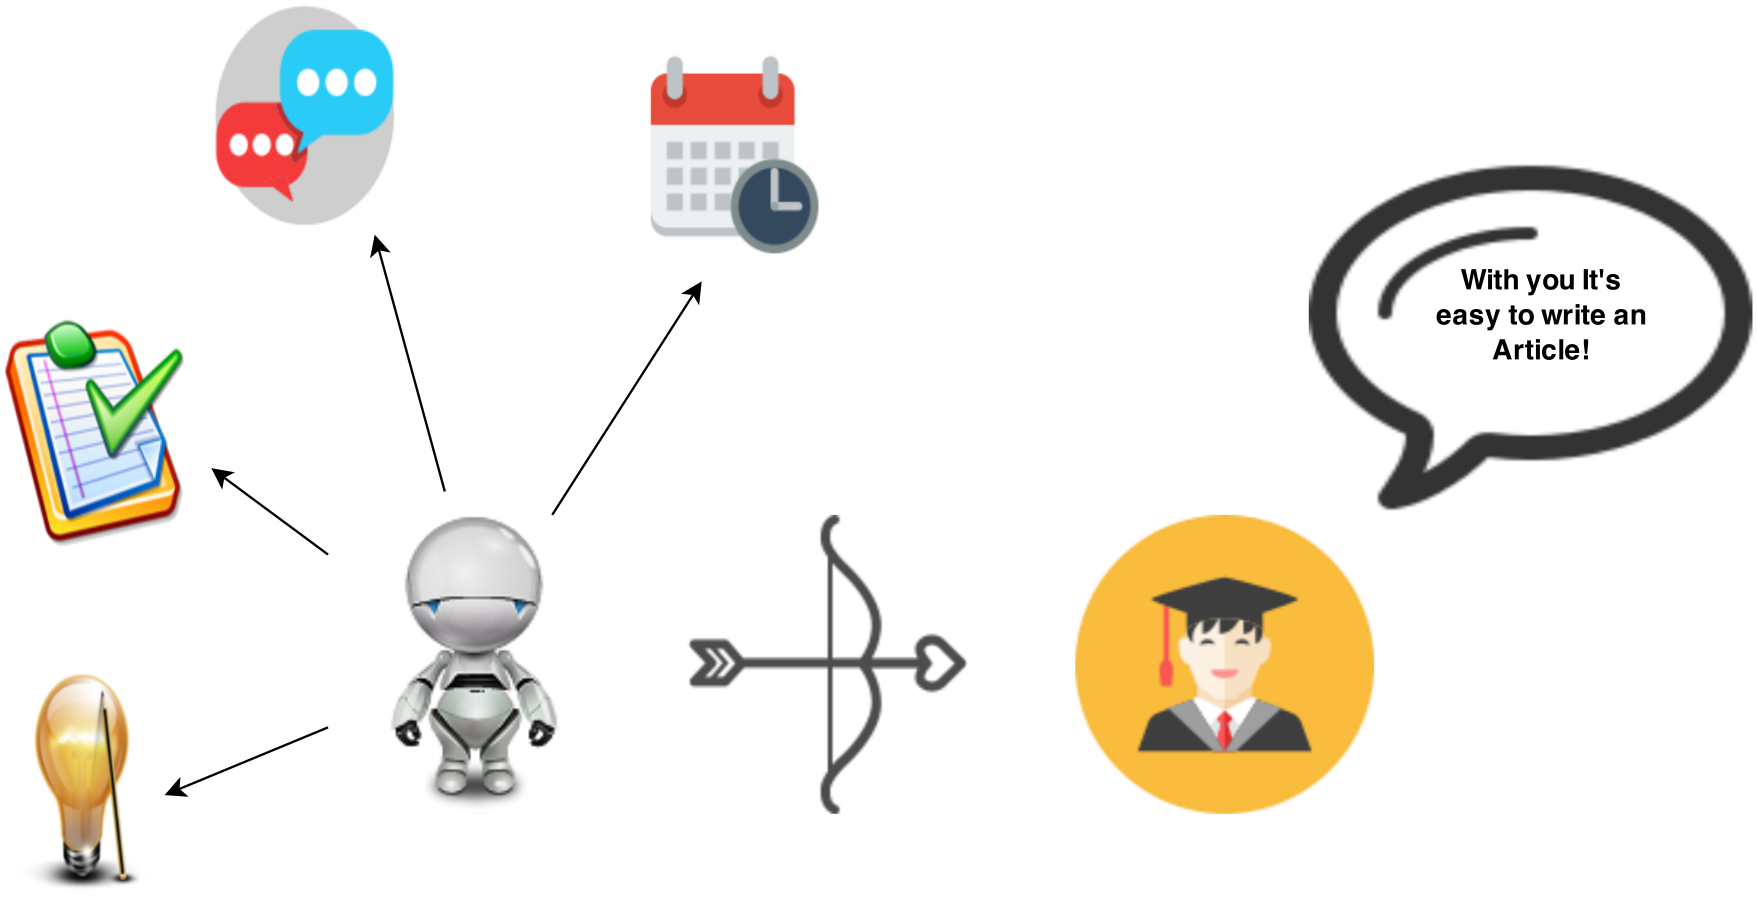
\includegraphics[scale=0.16]{./images/va.png}
\end{frame}

%Outline
\begin{frame}\frametitle{Outline}
	\begin{itemize}
		\item Research 
		\item Technologies
		\item Design Architecture
		\item Features
		\item Metrics  \& Evaluation
		\item Demo
		\item Q\&A Session
	\end{itemize}
\end{frame}

%Research-Analysis
\begin{frame}\frametitle{Research}\framesubtitle{Analysis}
\begin{itemize}
	\item Domain analysis : the problem, project stakeholders
	\item Defining client requirement: interview , meetings with project owner, etc
	\item Translating : Client requirements to functional \& technical requirements
	\item Benchmarking tools: Framework, Methodologies 
\end{itemize}
	
\end{frame}
%Research-SETUP
\begin{frame}\frametitle{Research}\framesubtitle{Set up}
\begin{itemize}
	\item Scrum: roles, sprint, etc
	\item Tools: Framework, installations, Github
	\item Organization : Trello 
	\item Project planning
\end{itemize}
	
\end{frame}

%Technologies
\begin{frame}
\frametitle{Technologies}
\centering

\includegraphics[scale=0.37]{./images/presentation_techlogos.png}
\end{frame}
%Design1-MVC
\begin{frame}
\frametitle{Design}\framesubtitle{Model View Controller}
\centering
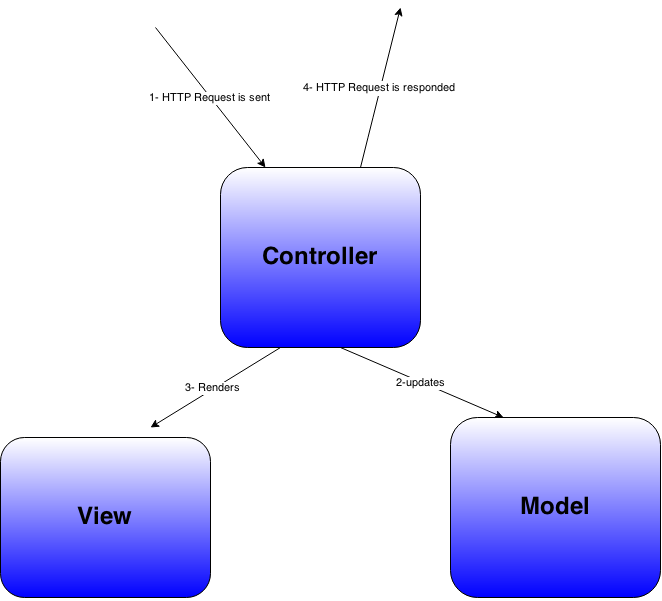
\includegraphics[scale=0.26]{./images/MVCdiag.png}
\end{frame}
%Design1-rma

\begin{frame}
\frametitle{Design}\framesubtitle{Relational Model}
\centering
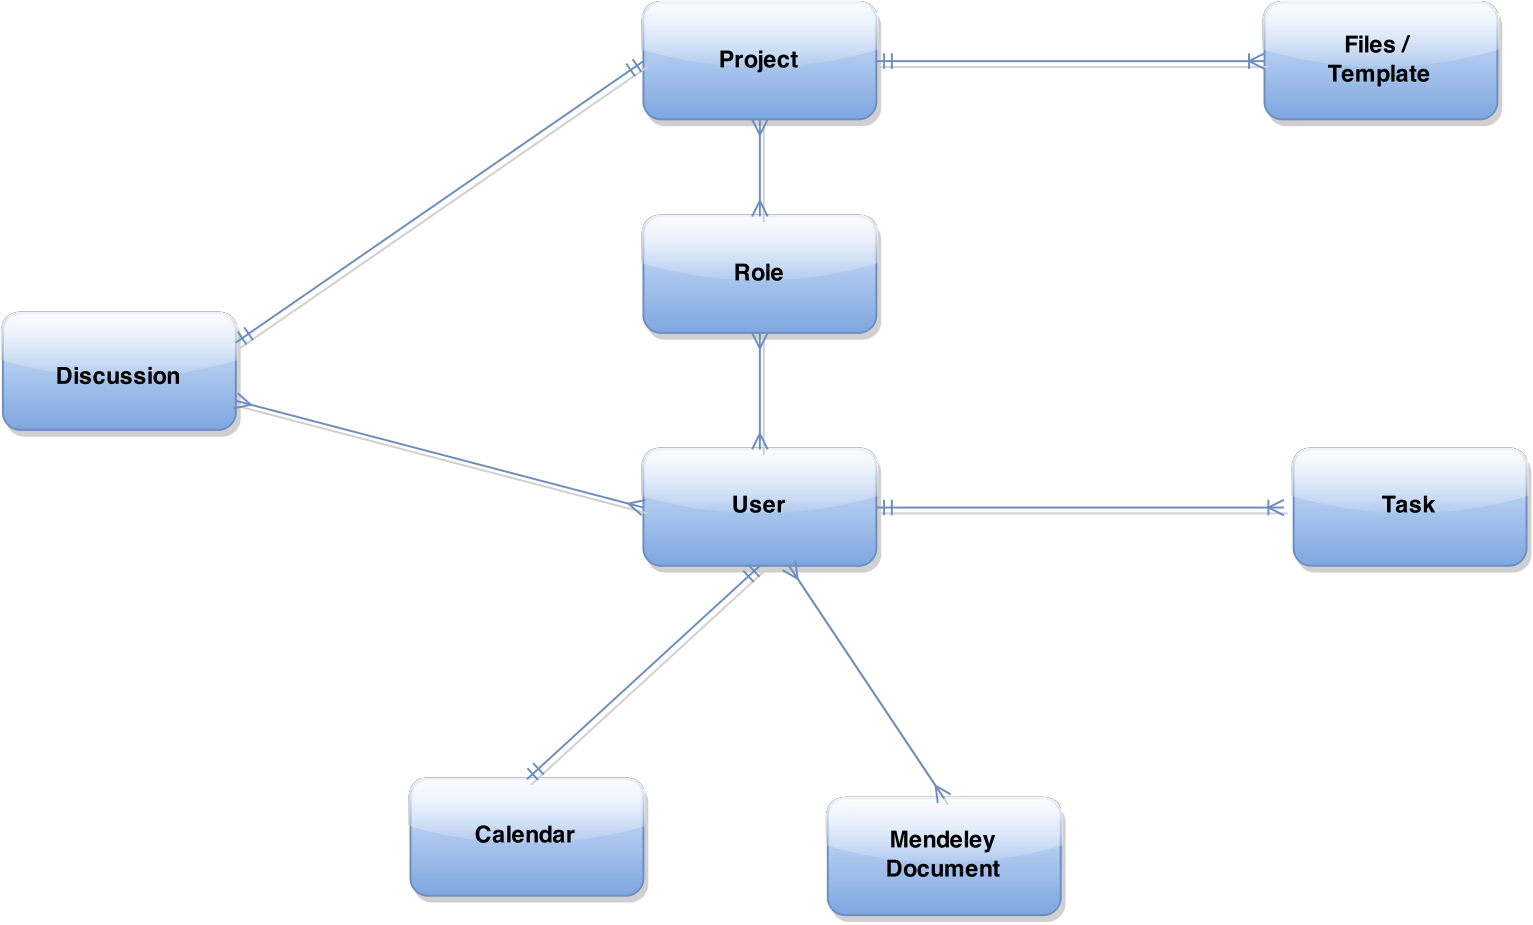
\includegraphics[scale=0.2]{./images/RMA.png}
\end{frame}
\begin{frame}\frametitle{OAuth2 Authentication}
	\begin{itemize}
		\item Allowing users to authenticate themselves through accounts from other web-services
		\item Google Plus and Mendeley
		\item Use of existing Google Plus OAuth2 library
		\item Extended library for Mendeley
		\item Library can also be used for Facebook, Twitter, GitHub,...
	\end{itemize}
\end{frame}



\end{document}
